%!TEX root = ../../main.tex

\chapter{Modellhafte Darstellung zur Evaluierung}

\section{Versuchsaufbau}

\subsection{Motorenmodell}

\subsection{Hardwaremodell}
\label{subsec:hardwaremodell}

\section{Technische Umsetzung}

\subsection{Detektion des Propellerblattes}
Um neben einer Umwuchtdetektion auch eine Umwuchtlokalisierung zu ermöglichen, ist die Detektion mindestens eines Propellerblattes zwingend notwendig.
Zwingend notwendig ist dies, da der Arduino für die lokalisierung der Unwucht die Unwuchtmessung jeweils pro vollständiger Umdrehung ($360^\circ$ Umdrehung) des Propellers starten muss.
Durch die Detektion beider Propellerblätter würden sich Vorteile bei der Zuordnung der Messergebnisse der Unwucht ergeben. 
Da sich dies jedoch, wie in den follgenden Kapiteln aufgezeigt wird, aufgrund der technischen Umsetzung als problematisch herrausstellt und durch die Detektion eines Propellerblattes und der Umdrehungsgeschwindigkeit des Propellers Rückschlüsse auf das zweite Propellerblatt gezogen werden können, wird im Zuge dieser Studienarbeit auf die Detektion des zweiten Propellerblattes verzichtet.

\subsubsection*{Theoretische Vorgehensweise}
Für die Detektion des Propellerblattes wurden zwei technische Lösungen erarbeitet, welche im späteren Verlauf dieses Kapitels gegenüber gestellt werden.
Beiden Lösungen liegt jedoch die gleiche theoretische Vorgehensweise zugrunde:
\begin{enumerate}
	\item Eine Seite des Propellers schwarz anmalen / schwarz bekleben
	\item Propeller mit definierter Drehzahl rotieren lassen
	\item Bei Detektion der schwarzen Fläche Interrupt auslösen
\end{enumerate}


\begin{figure}[h]
	\centering
	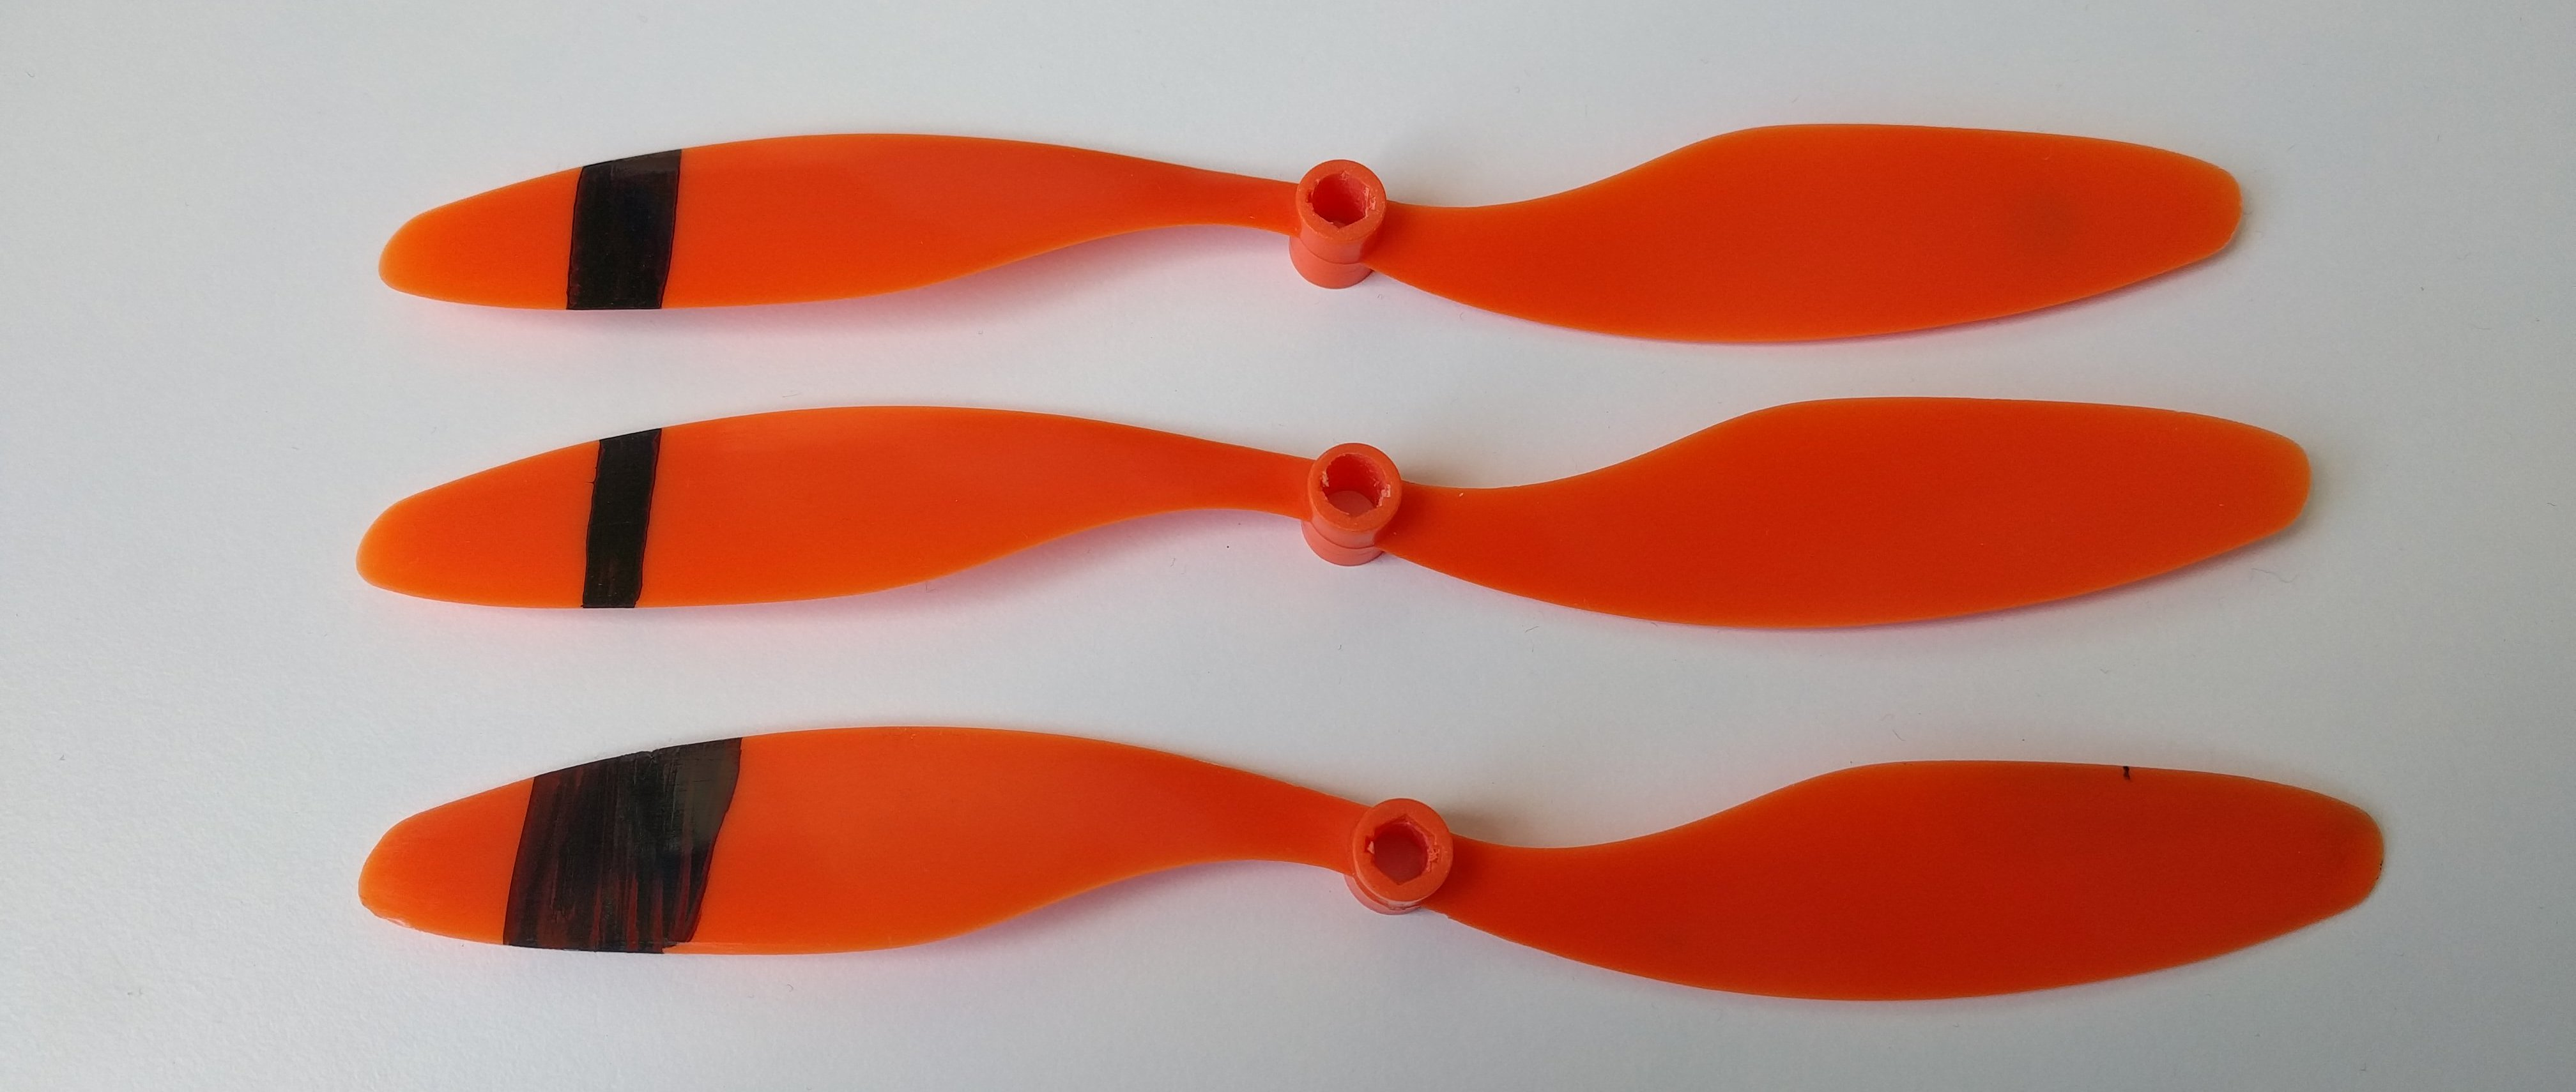
\includegraphics[width=.9\textwidth]{chapter/03/propeller_detektion.jpg}
	\caption{Modifikation zur Detektion eines Propellerblattes}
	\label{fig:propeller_detektion}
\end{figure}
Wie in Abbildung \ref{fig:propeller_detektion} erkennbar ist, gestaltet sich die Detektion des zweiten Propellerblattes als schwierig. 
Um das Propelerblatt für den Sensor erkennbar zu machen, müsste es auf der zweiten Seite ebenfalls schwarz bemahlt bzw. beklebt werden.
Dies würde jedoch dazu führen, dass bei laufendem Motor zwar zwischen beiden Propellerblättern unterschieden werden kann (jedes zweite erkannte Propellerblatt ist das gleiche), jedoch keine verlässliche Aussage möglich ist, an welchem der beiden Propellerblätter die Unwucht letztlich wirklich ist, da der Sensor nicht wirklich eindeutig zwischen den Propellerblättern unterscheiden kann.
Denn selbst die Unterscheidung der Propellerblätter bei laufendem Motor nicht sehr zuverlässlich.
Kommt es beispielsweise zu einem Messfehler - bedingt durch Lichteinflüsse oder änlichem - kann es passieren, dass ein Propellerblatt nicht erkannt respektive übersprungen wird.
Wird die Messung mit nur einm bemalten bzw. beklebten Propellerblatt durhgeführt und durch einen Messfehler nicht erkannt, ist die Messung bis zur nächsten Detektion prinzipiell falsch, kann aber später als Ausreiser ignoriert werden.
Werden jedoch beide Seiten bemalt bzw. beklebt und eine der beiden Seiten wird übersprungen, verschiebt sich die Position des Propellerblattes für die restliche Messung.
Dies würde zu einem vollkommen falschen Merrergebnis führen.
Falsche Werte könnten nicht mehr als Ausreiser aussortiert werden, da diese ab dem Zeitpunkt des Messfehlers bis zum Zeitpunkt des nächsten Messfehlers bzw. bis zum Ende der Messung perse richtig wären, jedoch um 180$^\circ$ verschoben.

\subsubsection*{Vergleich zwischen Sensoren}
Zur Detektion des Propellerblattess stehen zwei verschiedene Arten an Sensoren zur Auswahl, welche im follgenden gegenübergestellt und bewertet werden.

\newcolumntype{M}{>{\centering\arraybackslash}X}
\begin{table}[h]
	\centering
	\begin{tabularx}{0.95\textwidth}{M|M}

		Lichtsensor & IR-Reflektions-Sensor \\
		\hline
		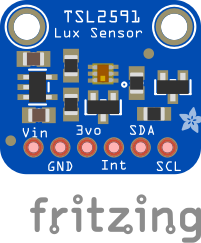
\includegraphics[height=3cm]{images/chapter/03/sensor_tsl2591.jpg} & 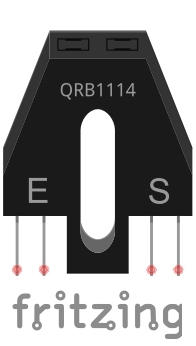
\includegraphics[height=4cm]{images/chapter/03/sensor_ir.jpg}  \\
		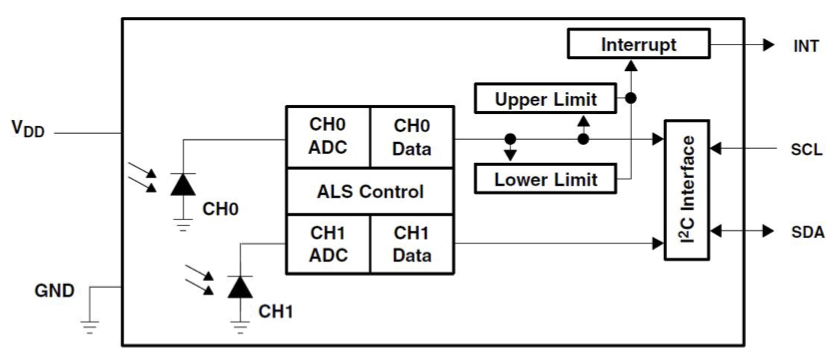
\includegraphics[height=3cm]{images/chapter/03/sensor_tsl2591_schema.png} & 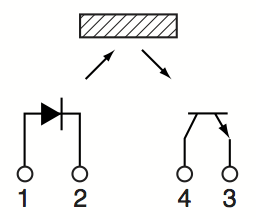
\includegraphics[height=3cm]{images/chapter/03/sensor_ir_schema.png} \\
		Adafruit TSL2591 & Adafruit Reflective IR Sensor \newline \\
	\end{tabularx}
	\caption{Vergleich zwischen zwei verschiedenen Arten an Sensoren zur Detektion des Propellerblattes}
\end{table}
\todo{wohin mit den quellenverweisen der zwei unteren Bildern}

Wie bereits beschrieben, arbeiten beide Sensoren auf gleiche Art und Weise - durch Detektion einer schwarzen Fläche. 
Allerdings ergeben sich durch die technologischen Unterschiede diverse Aspekte welche für bzw. gegen eine Verwendung sprechen.
Neben der Differenzierung zwischen Infrarotem Lichtspektrum und sichtbarem Lichtspektrum bei der Messung, wiest der Lichtsensor auch eine sehr hohe Lux Reichweite auf.
\todo{Quelle?} 
\begin{figure}[H]
	\centering
	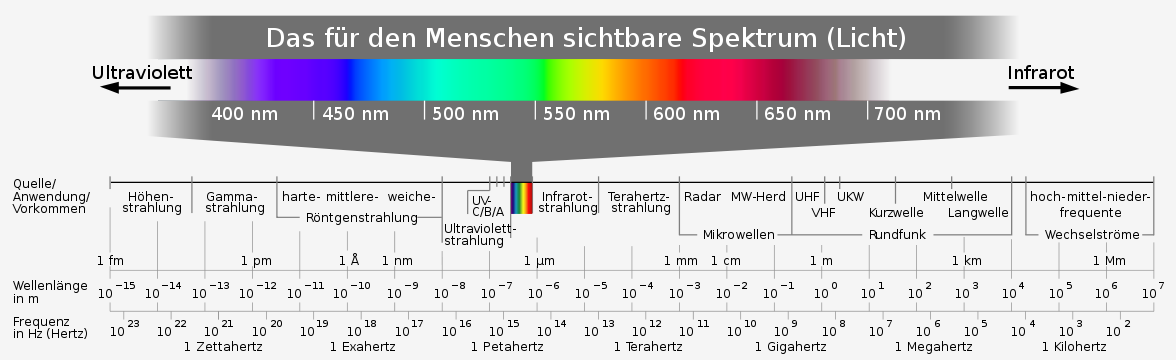
\includegraphics[width=\textwidth]{images/chapter/03/lichtspektrum.png}
	\caption{Darstellung des gesamten Lichtspektrums \cite[]{light_spectrum}}
\end{figure}
Hierduch können störhafte Lichteinflüsse wie z.B. durch sehr helle Sonneinstrahlung vermieden werden.
Dies erlaubt den Einsatz des Lichtsensors in nahezu allen Lichtverhältnissen - ein nicht zu vernachlässigender Aspekt, da hierdurch die Unwuchtmessung am realen Flugzeugmotor nicht zwingend in einer Umgebung mit kontrolierbaren Lichteinflüssen wie beispielsweise einem Hangar stattfinden muss.
Desweiteren bietet der Lichtsensor eine integrierte Interrupt Schnnittstelle, wodurch die Komplexität deutlich reduziert werden könnte im Vergleich zu einem \ac{IR}.
Trotz der Tatsache, dass der Lichtsensor in den soeben beschriebenen Aspekten einem \ac{IR} deutlich überlegen ist, bietet dieser deutliche Vorteile, welche letztlich ausschlaggebend ist für die Entscheidung welcher der beiden Sensoren verwendet werden soll.
Durch die technische Beschaffenheit des \ac{IR} im Vergleich zum Lichtsensor ist ein deutlich einfacherer Aufbau im Vergleich zum Lichtsensor möglich.
Der wichtigste Aspekt hierbei ist jedoch die deutlich höhere Abtastrate des \ac{IR} im Vergleich zum Lichtsensor. 
\begin{figure}[H]
	\centering
	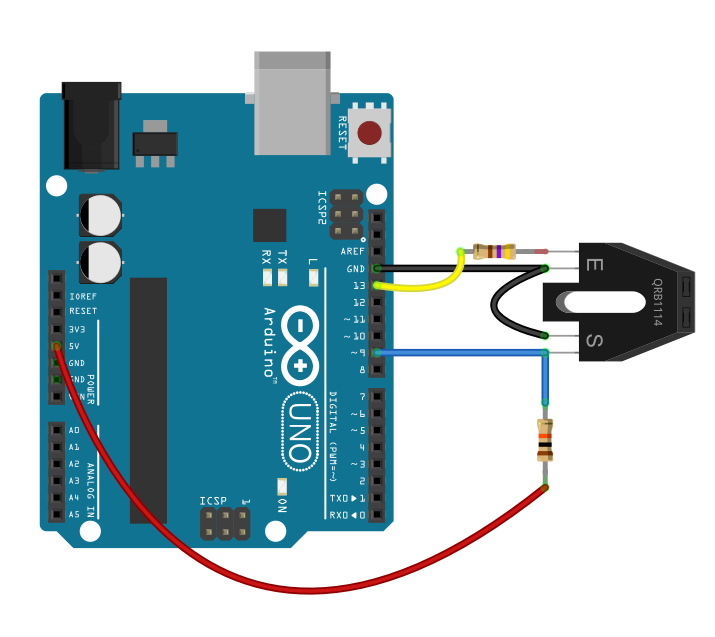
\includegraphics[width=0.75\textwidth]{images/chapter/03/sensor_ir_schaltung.png}
	\caption{Beispielhafte Verwendung des \ac{IR}s \cite{sensor_ir_schaltung}}
	\label{fig:ir_example}
\end{figure}
Abbildung \ref{fig:ir_example} stellt eine exemplarischen Verwendungszweck des \ac{IR}s dar. 
Der Sensor (in Abbildung \ref{fig:ir_example} durch ein S repräsentiert) ist sowohl direkt mit dem Arduino als auch mit einem Pull-Up Wiederstand verbunden.
Dies hat zur Folge, dass am Arduino Port 5V anliegen, solange der Sensor eine Reflexion des vom Emitter (In Abbildung \ref{fig:ir_example} durch ein E repräsentiert) ausgesendeten Lichtes erhält.
Wird das Licht nicht reflektiert - dies ist der Fall sobald sich die schwarze Fläche des Propellerblattess vor dem \ac{IR} befindet - liegt am Arduino Port 0V an.
Für die Detektion des Propellerplattes - respektive für den Wechsel zwischen 5V und 0V - wird auch als Rise bzw. Fall-Time bezeichnet - benötigt der \ac{IR} lediglich eine Zeit von 8$\mu$s ausgehend einer Temperatur von 25$^\circ$C \cite[S.2]{ir_datasheet}.
\todo{Quelle angeben wo des mit den 8 mus herkommt}
\todo{Bild des Andreas ans Whiteboard gemalt hat reinpacken}
Der Lichtsensor hingegen integriert alle gemessenen Werte über einen zuvor definierten Zeitraum. Das Problem hierbei ist, dass dieser Zeitraum lediglich auf die folgenden Werte gesetzt werden kann \cite[S.13]{tsl2591_datasheet}:
\begin{itemize}
	\item 100ms
	\item 200ms
	\item 300ms
	\item 400ms
	\item 500ms
	\item 600ms
\end{itemize}
Ein Flugzeugmotor dreht im Leerlauf mit ca. 2500 U/s. Um ein valides Ergebniss zu erziehlen, muss die minimale Abtastrate höher als die maximale Umdrehungszahl des Motors sein, um sicherzustellen, dass der schwarz markierte Bereich des Propellerblattess auch detektiert wurde.
Umgerechnet bedeutet dies, dass der Propeller für eine Umdrehung ca. 24ms benötigt.
Da die geringste Abtastrate des Lichtsensors jedoch 100ms beträgt, ist dieser für den Anwendugsfall dieser Studienarbeit ungeeignet.
Neben der Abtastrate ist auch die Integration der gemessenen Werte ein Problem. 
Da die schwarze Fläche des Propellerblattess deutlich kurzere Zeit vor dem Sensor ist als dies nicht der Fall ist würde eine aufintegration die kurze Zeit, die sich der Propeller vor dem Sensor befindet deutlich geringer ins Gewicht fallen als die zeit in der er sich nicht vor dem Sensor befindet.
\todo{umvormulieren}
Aus diesen Gründen wurde für die Umsetzung dieser Studienzeit auf den \ac{IR} als Sensor zur Detektion des Propellerblattes gesetzt.



% links
% tsl schema: aus pdf https://cdn-shop.adafruit.com/datasheets/TSL25911_Datasheet_EN_v1.pdf
% ir schema: aus pdf https://www.sparkfun.com/datasheets/Sensors/QRB1114.pdf
% lichtspektrum grafik https://de.wikipedia.org/wiki/Ultraviolettstrahlung#/media/File:Electromagnetic_spectrum_c.svg
% ir schaltung https://cdn-shop.adafruit.com/product-files/2349/pid2349.png

\subsubsection*{Probleme bei der Detektion des Propellerblattes mit einem \ac{IR}}
Aufgrund der technischen Beschaffenheit des \ac{IR}s ist eine Detektion des Propellerblattes in der Theorie ohne weiteres möglich.
Die Praxis zeigt jedoch, dass hierbei einige Probleme auftreten können.

Ein Problem des \ac{IR}s ist der benötigte Abstand zwischen Sensor und Propellerblatt von minnimal 2mm bis maximal 10mm, sowie der richtige Winkel zum Propellerblatt.
\todo{Woher kommt die Info??}
Es reicht jedoch leider nicht aus, den Sensor fix an einer Stelle zu befestigen, da sich durch die Fliehkräfte der gewichteten Propellerblätter (Gewichte wurden verwendet um Unwucht zu erzeugen - hierauf wird in Kapitel \ref{subsec:detektion_der_unwucht} genauer eingegangen) der Abstand zwischen Propellerblatt und Sensor verändert.
\begin{figure}[H]
	\centering
	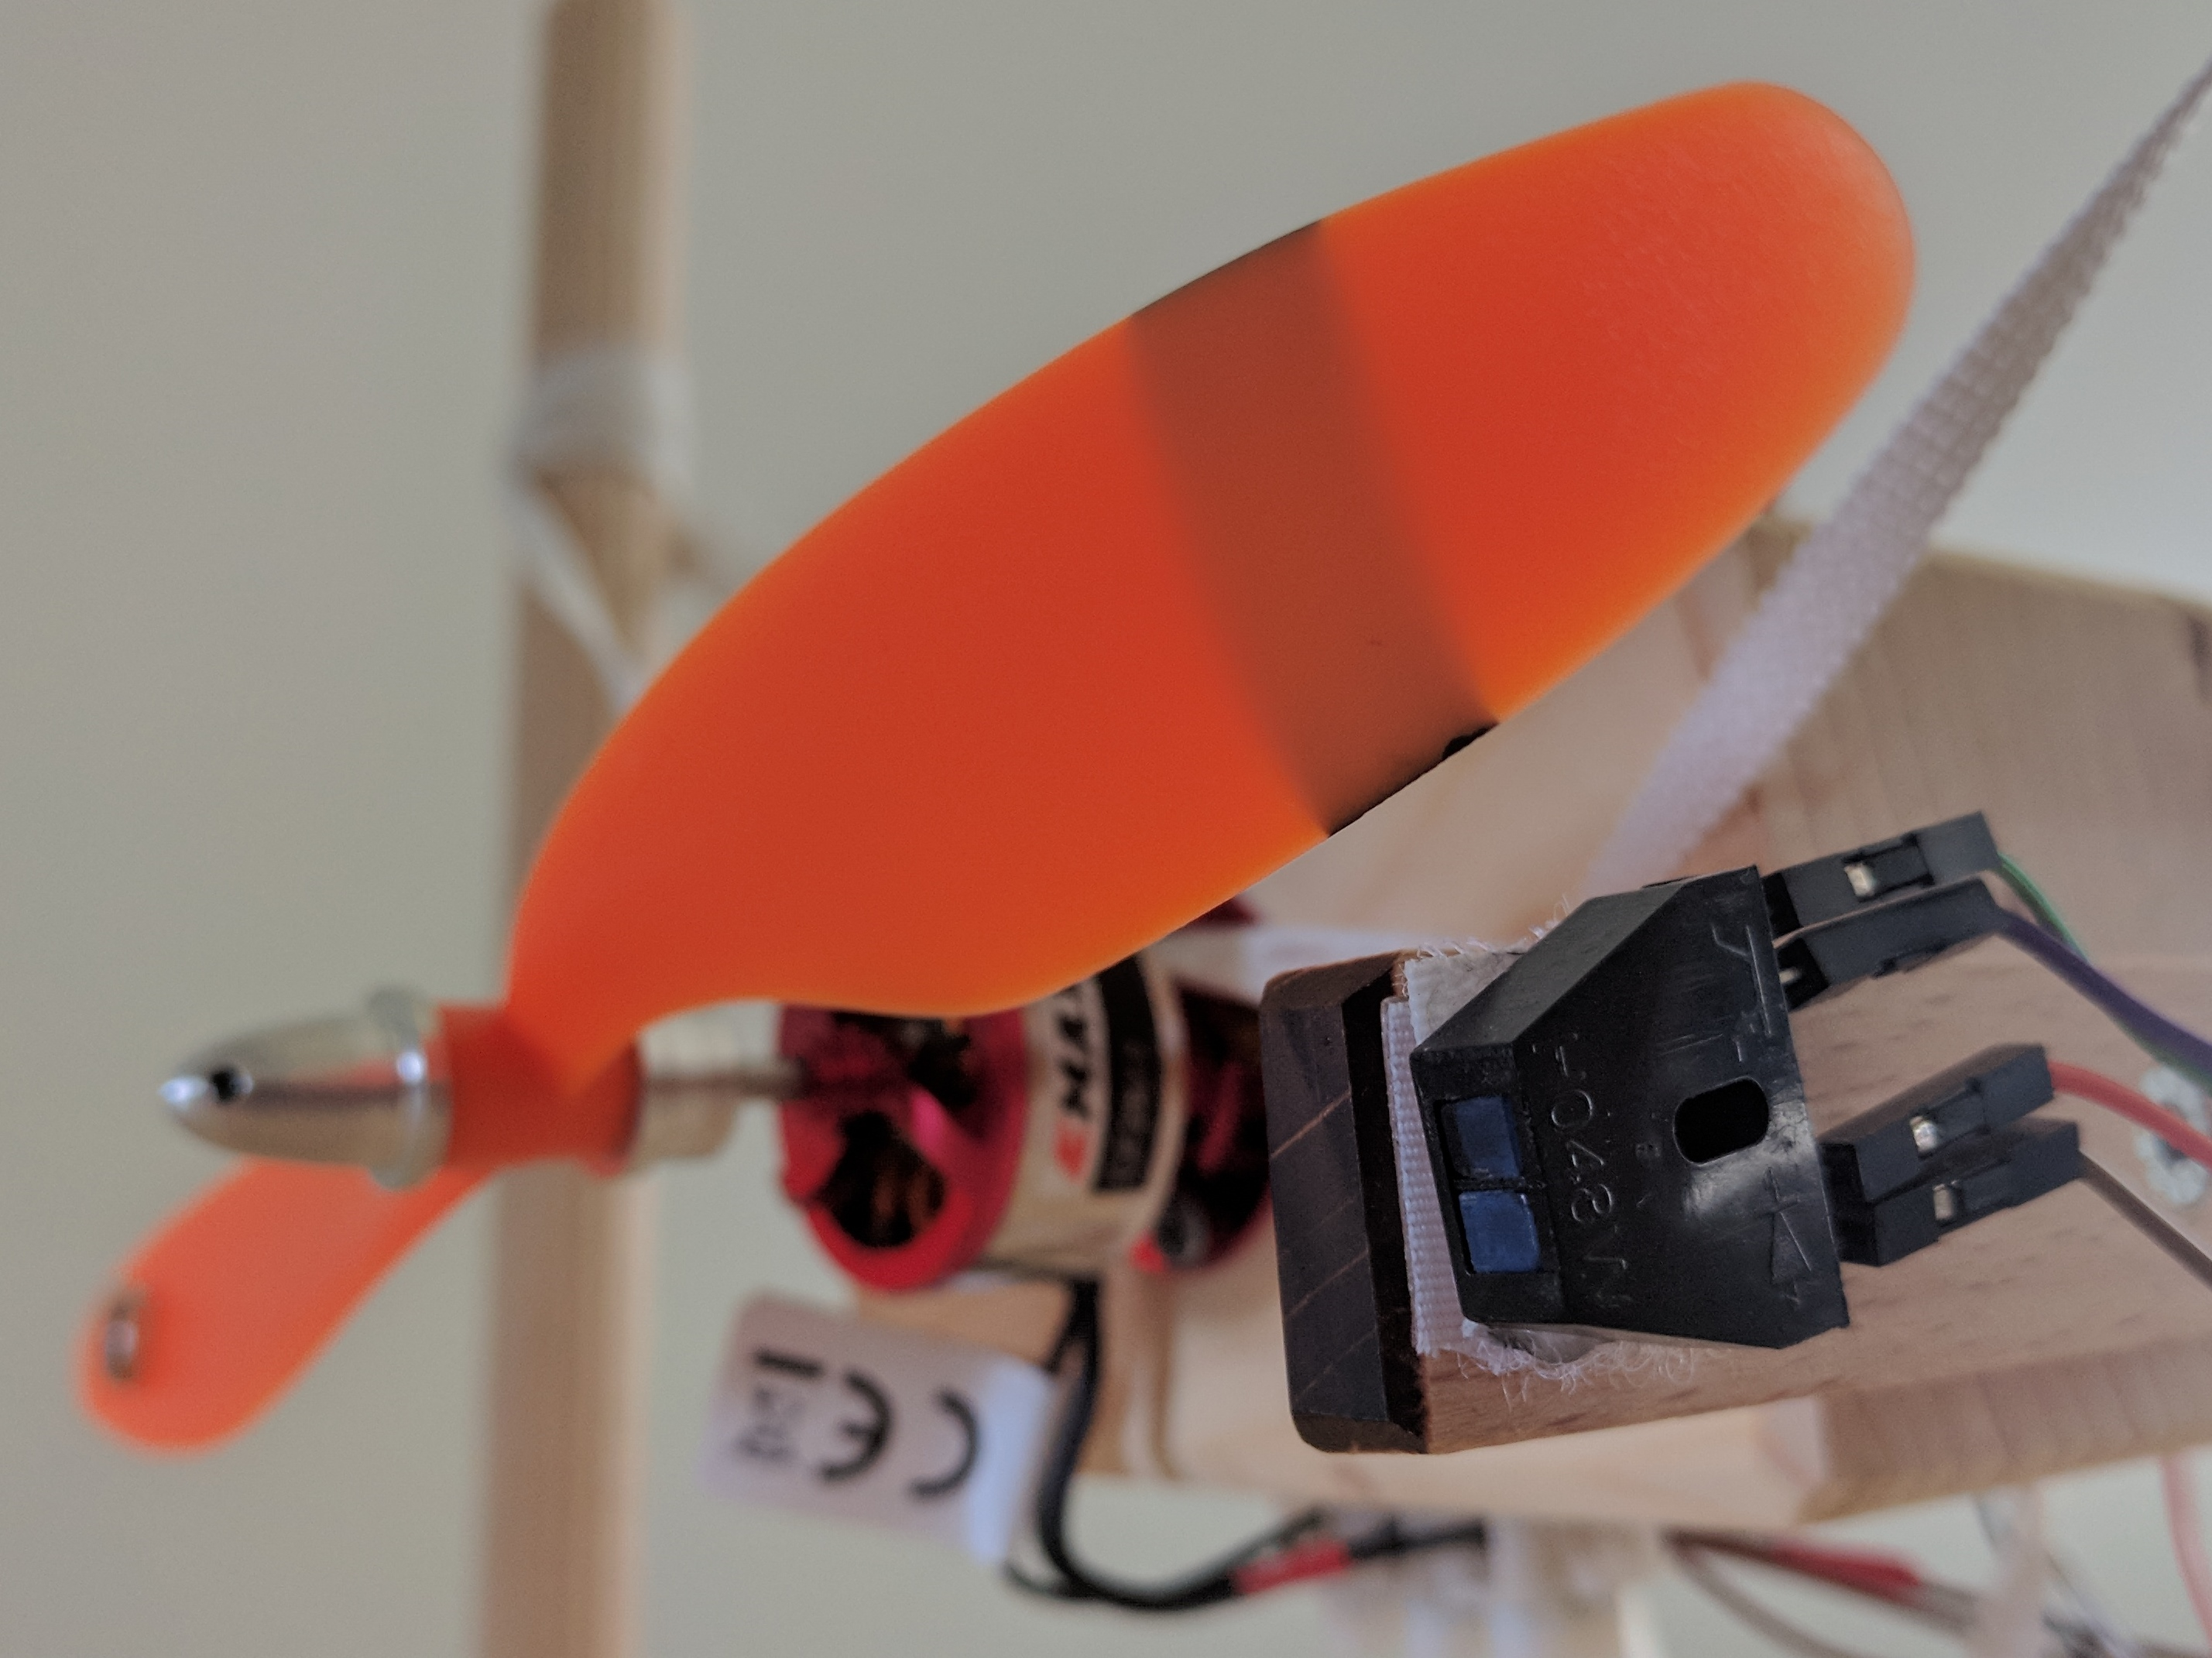
\includegraphics[width=0.9\textwidth]{images/chapter/03/exp_ir_sensor.jpg}
	\caption{Befestigung des Sensors mithilfe eines Klettbandes}
	\label{fig:exp_ir_sensor}
\end{figure}
Aus diesem Grund wurde die Holzkonstruktion mit einem Klettband versehen, wie in Abbildung \ref{fig:exp_ir_sensor} zu sehen ist.
Dies ermöglicht es, den Sensor für jeden Propeller individuell einzustellen.

Neben dem Abstand bzw. dem Winkel des \ac{IR}s spielen jedoch auch die Lichteinflüsse eine Rolle.
Im Gegensatz zum Lichtsensor ist der \ac{IR} extrem anfällig gegenüber auf den Sensor einströmendes Licht.
Dies hat zur Folge, dass der Versuch nur in einer Umgebung mit kontrollierten Lichteinflüssen funktionieren kann.
Aufgefallen ist dieses Problem im Kontext dieser Studienarbeit, sobald sich der Sensor direkt vor einem Fenster mit Blickrichtung auf dieses befand.
Jedoch ist auch zu geringes Licht ein Problem, da hier der \ac{IR} die schwarze Fläche des Propellerblattes nicht mehr zuverlässig detektieren kann.

Das größte Problem stellt jedoch die kombination, der in Kapitel \ref{subsec:hardwaremodell} bewusst auf zwei Arduinos aufgeteilten Sensoren, bestehend aus einem \ac{9-DOF} - dieser wird in Kapitel \ref{subsec:detektion_der_unwucht} näher beleuchtet - und einem \ac{IR}, an einem einzigen Arduino dar.
\begin{figure}[H]
	\centering
	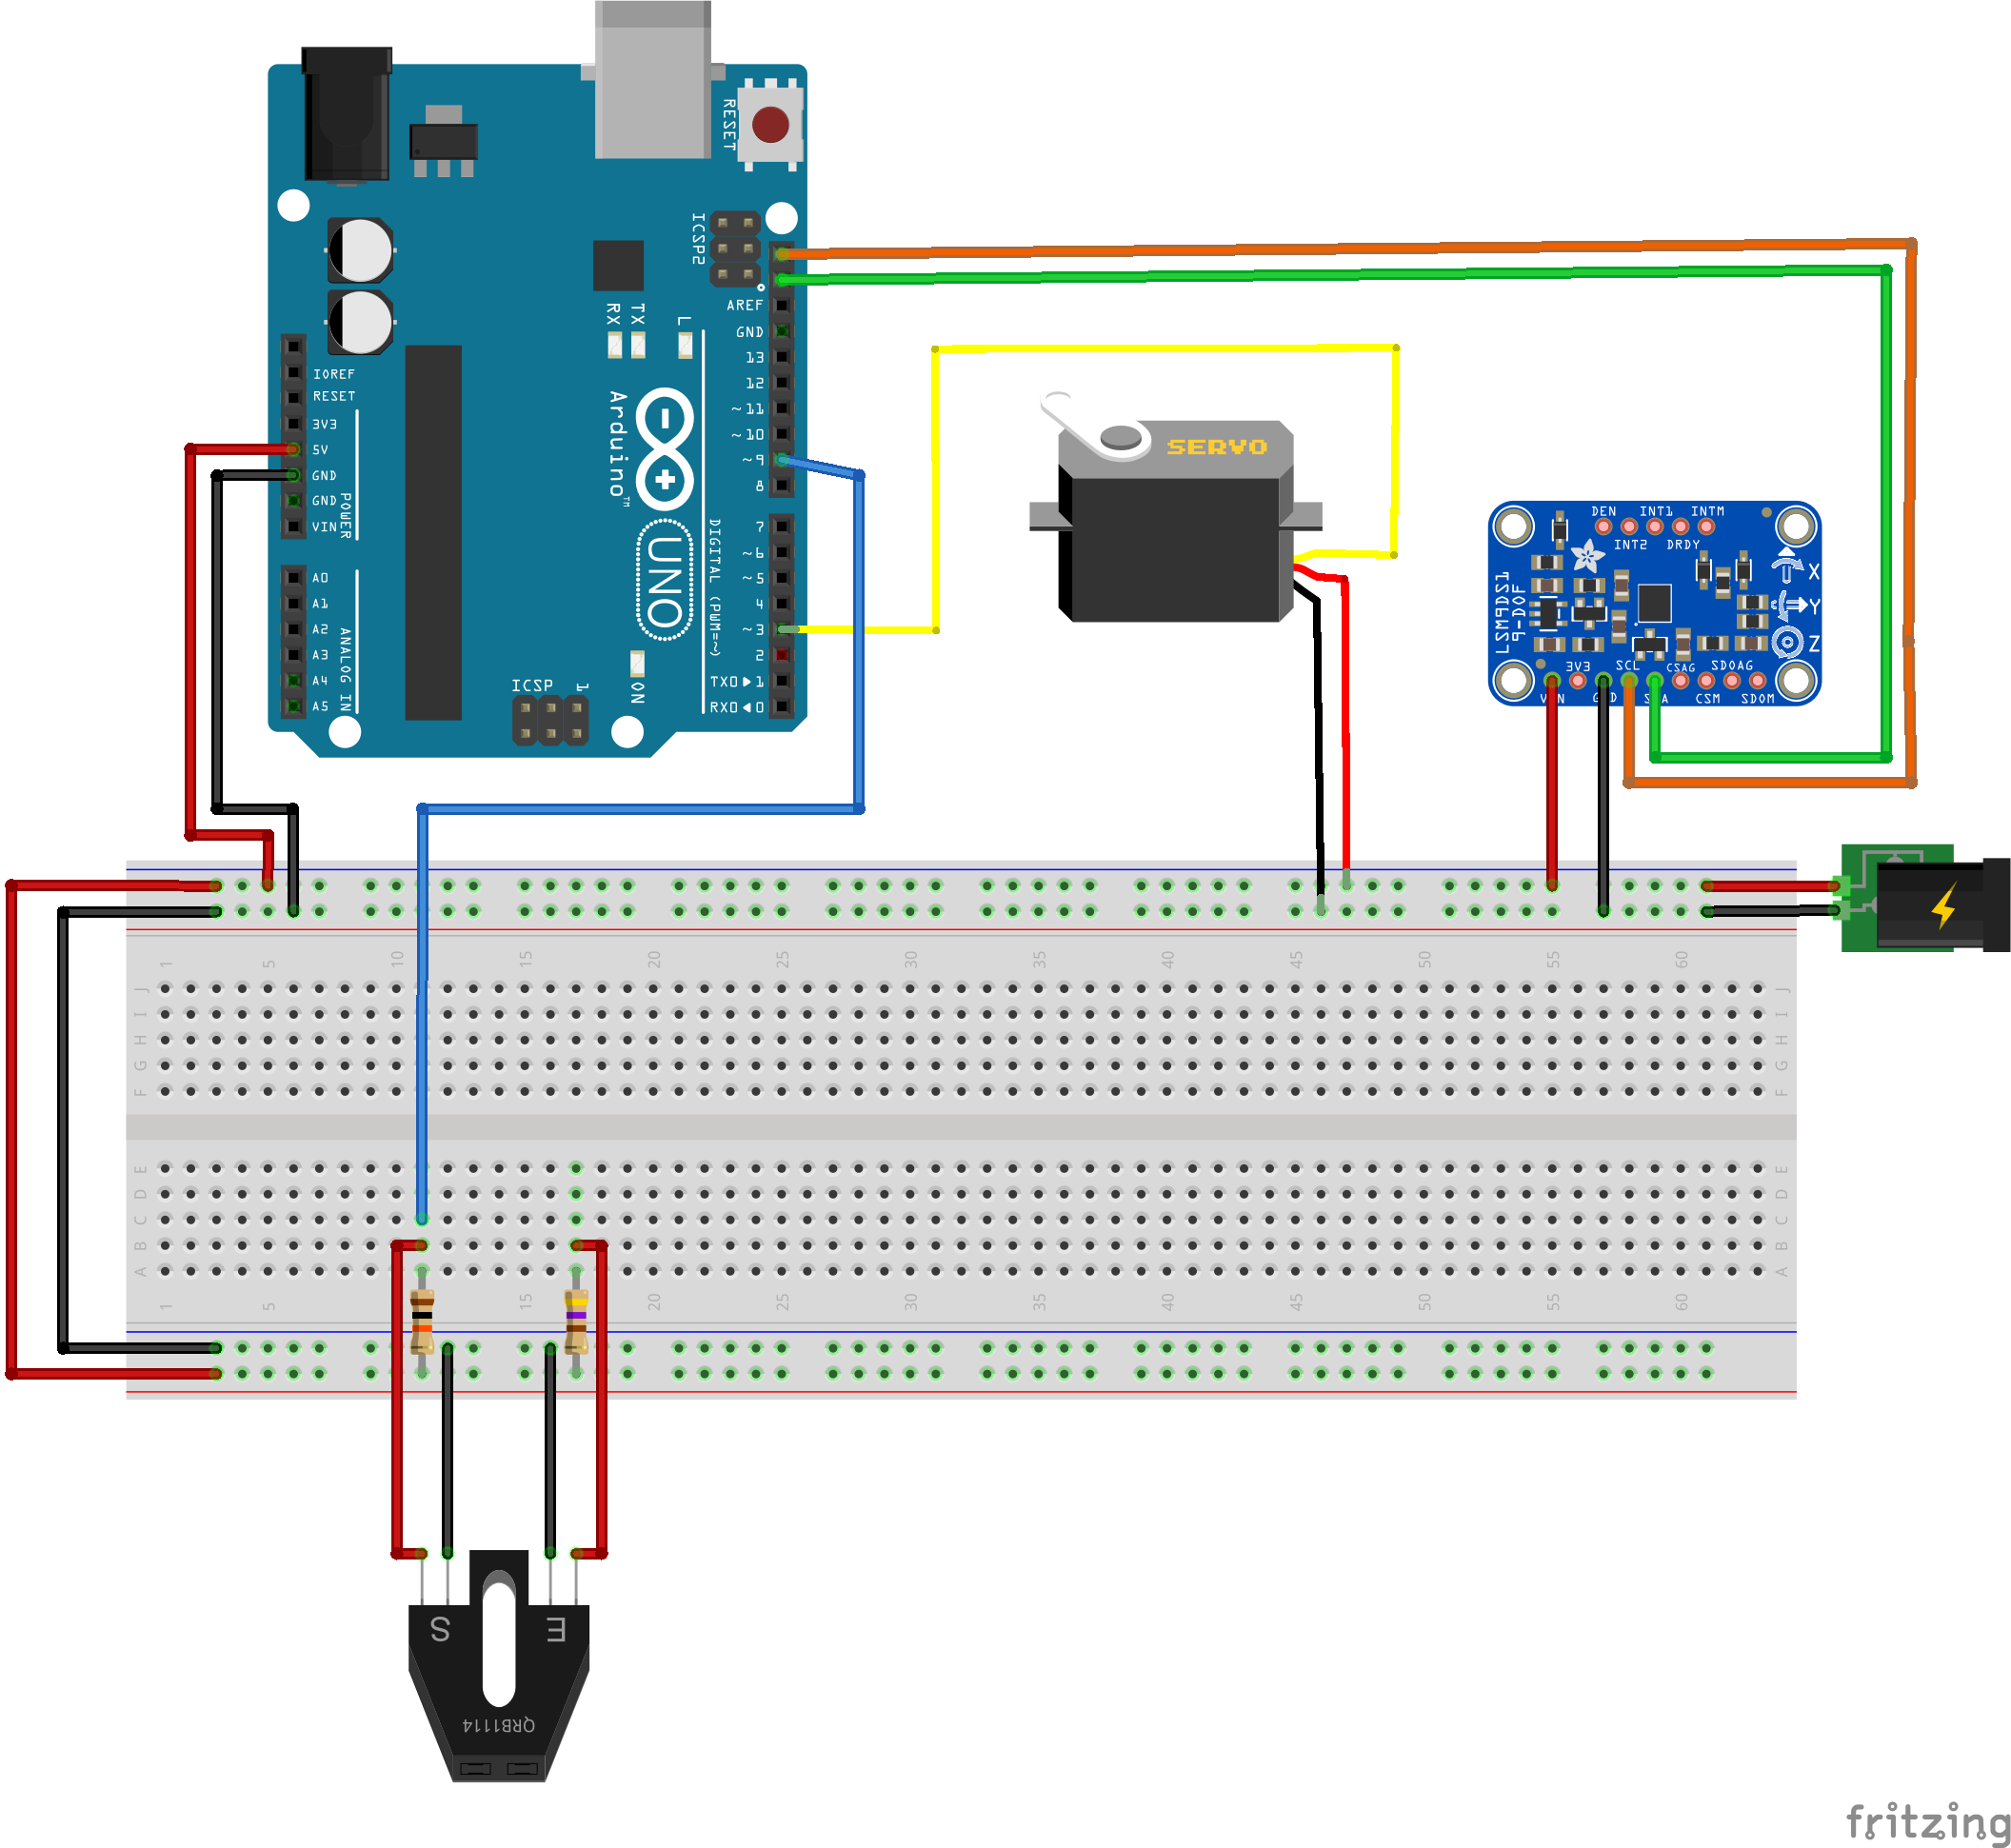
\includegraphics[width=0.9\textwidth]{images/chapter/03/hardware-layout-with-one-arduino.png}
	\caption{Altes Hardwaremodell mit einem Arduino}
\end{figure}
Bei gelichzeitigem Messen beider Sensoren ist eine zuverlässige detektion des Rotorblattes nicht möglich.
Abbildung \ref{fig:interrupts_are_shit} stellt die Messergebnisse des \ac{IR}s graphisch dar.
\begin{figure}[H]
	\centering
	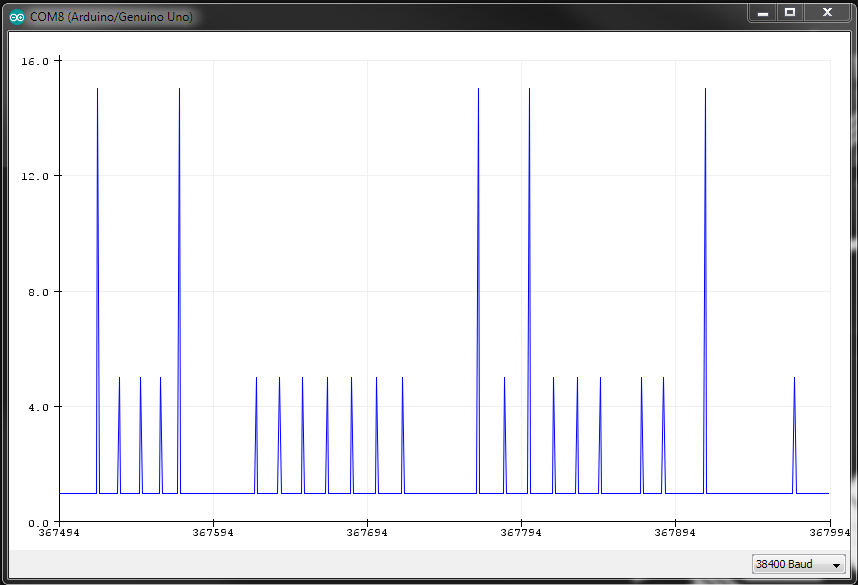
\includegraphics[width=0.9\textwidth]{images/chapter/03/interrupts_are_shit.png}
	\caption{Messwerte des \ac{IR}s bei gleichzeitiger Messung eines \ac{IR}s und eines \ac{9-DOF}s}
	\label{fig:interrupts_are_shit}
\end{figure}
Wie in Abbildung \ref{fig:interrupts_are_shit} zu erkennen ist, wurde das Propellerblatt nur unregelmäßig erkannt.
Desweiteren wurden teilweise auch Spiztenwerte von 15V gemessen, welche aufgrund der Stromversorgung von maximal 5V nicht vorkommen können.

Aus diesem Grund wurden die Sensoren auf die zwei Arudinos, \ac{A1} und \ac{A2} aufgeteilt (wie in Abbildung \ref{key} \todo{ref auf hardwaremodell bild setzen} dargestellt) und die Aufgaben entsprechend verteilt (wie in Abbildung \ref{fig:aufgaben-arduinos} dargestellt).
\begin{figure}[H]
	\centering
	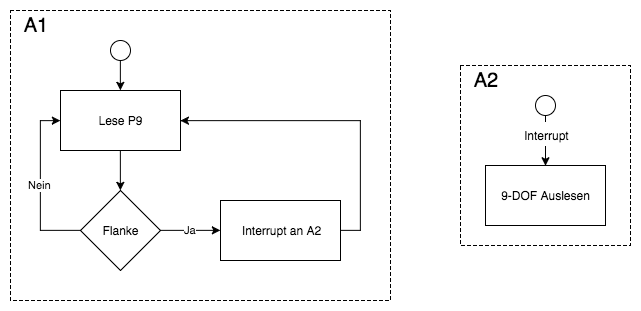
\includegraphics[width=0.9\textwidth]{images/chapter/03/aufgaben-arduinos.png}
	\caption{Aufgaben der beiden Arduinos \ac{A1} und \ac{A2}}
	\label{fig:aufgaben-arduinos}
\end{figure}
Durch die Trennung beider Sensoren und die Aufgabenteilung in Propellerblattdetektion und Unwuchtmessung ist \ac{A1} nun in der Lage das Propellerblatt konstant (im Rahmen einer gewissen Fehlertoleranz) zu detektieren.
\begin{figure}[H]
	\centering
	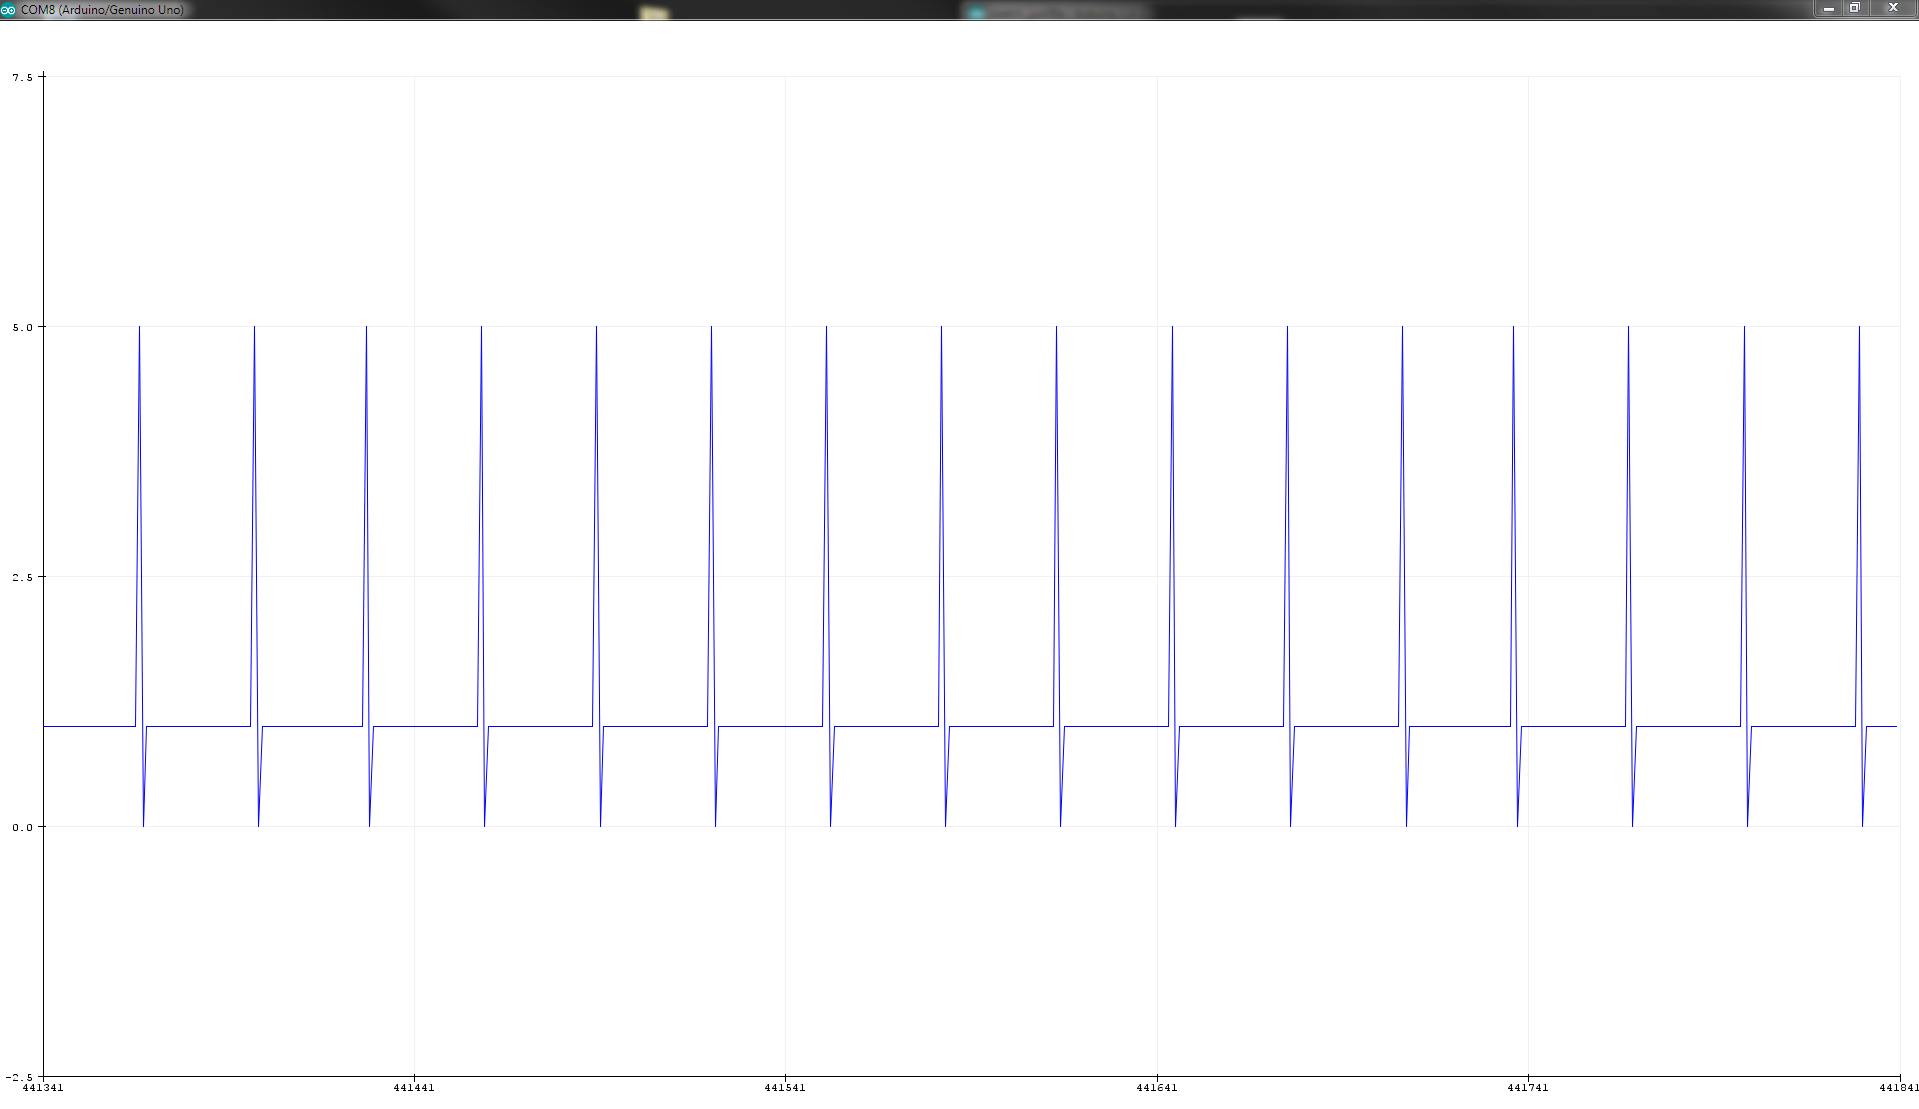
\includegraphics[width=0.9\textwidth]{images/chapter/03/self_made_interrupt_a1.png}
	\caption{Messerte des \ac{A1}}
	\label{fig:self_made_interrupt_a1}
\end{figure}
\todo{sollte hier noch der codesnippsel rein wie wir die selfmade interrupts erzeugt haben?}

\subsection{Detektion der Unwucht}
\label{subsec:detektion_der_unwucht}

\subsubsection*{Theoretische Vorgehensweise}
Aufgrund der Unwucht des Propellers entstehen Vibrationen am Motorblock
Durch Anbringung eines Sensors direkt am Motorblock können diese Vibrationen gemessen werden
Je nach Auslenkung des Motorblockes in Abhängigkeit von dem aktuell vorbeidrehenden Propeller sollten so Rückschlüsse auf die Herrkunft (also von welchem Propeller aus) der Unwucht getroffen werden können

\subsubsection*{Sensortechnologie}
Verwendeter Sensor: Adafruit LSM9DS1
Eingesetzter Sensor ist ein 9-DOF (\textbf{D}egrees \textbf{f} \textbf{F}reedom). Er ist mit 4 verschiedenen Sensoren ausgestattet. Darunter ein Beschleunigsungssensor welche die Beschleunigung des Sensors in drei verschiedene Richtungen misst, ein Gyroskop welcher die Ausrichtung des Sensors misst und ein Magnetometer welcher die Lage des Sensors in Abhängigkeit des Erdmagnetfeldes darstellen kann. Der vierte Sensor ist ein Temperatursensor, welcher für dieses Experiment jedoch irrelevant ist.

\subsubsection*{Messung der Unwucht}
Hier kommen dann Bilder rein und wir erklären und diskutieren die Ergebnisse dann, oder?

\subsubsection*{Probleme bei der Detektion}
Nachfolgende Probleme traten bei der Verwendung des Sensors auf:
- Das Auslesen der Sensordaten dauert zu lange. Es ist möglich 2-3 Messergebnisse (Variation hängt von Gewicht des Propellers ab) innerhalb einer Umdrehung (~20ms) des Propellers zu erhalten. Ein Versuch dieses Verhalten zu verbessern bestand darin die Verbindungsgeschwindigkeit zwischen \textit{Arduino} und Sensor zu erhöhen. Die Verbindung zwischen den beiden Geräten findet über die Schnittstelle I\textsuperscript{2}C im normalen Modus statt. Durch Manipulation der \textit{twi.h}, eine Header-Datei der Arduino-Bibliothek \textit{Wire.h}, welcher die Verbindungsparameter für die I\textsuperscript{2}C-Schnittstelle steuert, war es möglich die Verbindung im Fast-Mode zu betreiben. Damit wurde die Anzahl an Messergebnisse pro Umdrehung von 2-3 auf 3-5 Messungen erhöht. Dies ist aber weiterhin zu wenig um eine konkrete Entscheidung über die Lokalisation der Unwucht treffen zu können.
Es existiert eine weitere Möglichkeit den Sensor auf eine höhere Messrate zu bekommen, welche im Datenblatt jedoch nur sehr kurz und knapp erklärt ist. Hierbei ist es möglich das Gyroskop des Sensor abzuschalten und den Beschleunigungssensor mittels eines "Burst-Modus" (multiple reads) auszulesen. Den Sensor in diesen Modus zu setzen und auszulesen war allerdings aufgrund Mangel des technischen Verständnisses und der Datenblatterklärung nicht möglich.
Es kann davon ausgegangen werden, dass die benötigte Zeit für die Messung der Sensoren bei dem eingesetzten Sensor schon intern zu lange dauert. Die Empfehlung (für zukünftige Projekte ?) liegt daher auf dem Einsatz von anderen Sensoren, welche für diesen Einsatzzweck besser geeignet sind. Ein Beispiel hierfür ist der Bosch BMA180. Dies ist ein dreiachsichger Beschleunigungssensor, welcher intern mit einer Messgeschwindigkeit von 1200Hz operieren kann. Damit kommt dieser Sensor auf ein komplett neues Messergebniss alle 417$\mu$s (Quelle: http://irtfweb.ifa.hawaii.edu/~tcs3/jumpman/jumppc/1107-BMA180/BMA180-DataSheet-v2.5.pdf). Hiermit sind bei einer Umdrehungszeit von ~20ms bis zu 48 Messergebnisse möglich, welche wahrscheinlich ausreichend sind für eine Aussage über die Unwuchtlokalisierung. Eine weitere Möglichkeit für den Ersatz des Sensor wäre der Einsatz einer inertialen Messeinheit (englisch \textit{inertial measurement unit}, IMU). Dies ist meist eine räumliche Kombination von mehreren Sensoren, welche auch Einsatz in heutigen Drohnen finden. Ob sich diese für den hier benötigten Einsatz verwenden liesen ist nicht bekannt und müsste weiter recherchiert werden.
